\section{Einf�hrung}

\subsection{Motivation}

\begin{frame}{\insertsubsection}
  \begin{block}<+->{Messger�te liefern unzuverl�ssige Daten}
    \begin{itemize}
      \item GPS Tracker sind unzuverl�ssig in der N�he von Geb�uden
      \item Sensoren sind empfindlich gegen�ber �u�ere Einfl�sse
          \begin{itemize}
              \item Z.B. starker Fall der Temperaturen bei einem Windzug.
          \end{itemize}
    \end{itemize}
  \end{block}
\begin{figure}
    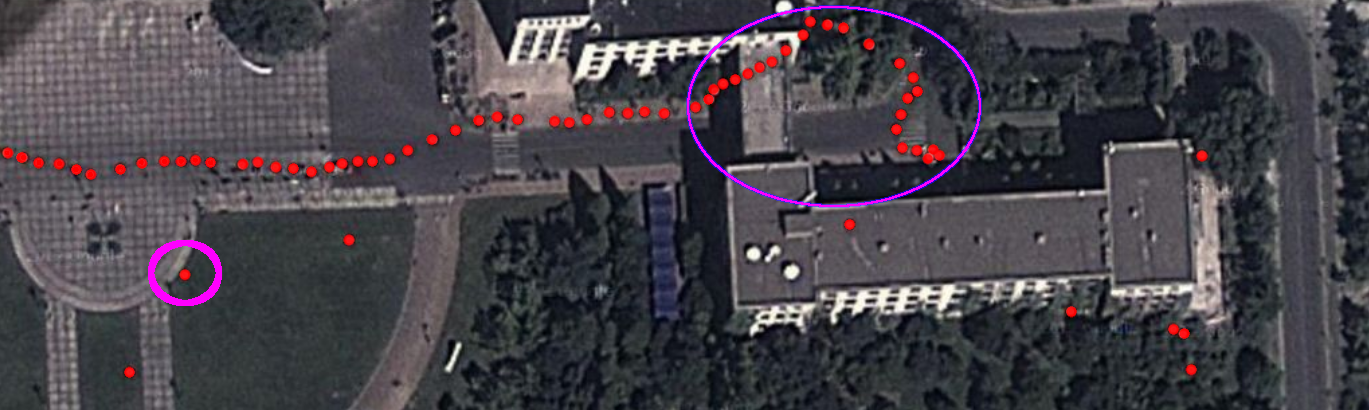
\includegraphics[width=\textwidth]{GPS_Motivation_Example.png}
    \caption{GPS-Tracking auf dem Campus der Tsinghua Universit�t \cite{Shaoxu17}}

\end{figure}

\end{frame}

\begin{frame}{\insertsubsection}
  \begin{block}<+->{Ans�tze mit den Umgang von unzuverl�ssigen Daten}
    \begin{enumerate}
        \item Unzuverl�ssige Datenpunkte mit der Anomalienerkennung entfernen
            \begin{itemize}
                \item Einzelne Ausrei�er werden entfernt  \neutranie
                \item Entfernen langer Folgen von Ausrei�er machen Ergebnis unbrauchbar \frownie
                \item Lange Folgen von Ausrei�er werden als solche ggf. nicht erkannt \frownie
            \end{itemize}
        \item Unzuverl�ssige Datenpunkte mit der Anomalienerkennung reparieren
            \begin{itemize}
                \item Einzelne Ausrei�er werden korrigiert \smiley
                \item Lange Folgen von Ausrei�er werden zu stark ver�ndert (widerspricht den Minimum-Change-Prinzip) \neutranie
                \item Lange Folgen von Ausrei�er werden als solche ggf. nicht ver�ndert \frownie
            \end{itemize}
    \end{enumerate}
  \end{block}
\end{frame}

\begin{frame}{\insertsubsection}
    \begin{block}<+->{Hinzunahme von als wahr markierte Werte}
    \begin{enumerate}
        \item Markierung durch den Benutzer
            \begin{itemize}
            \item Z.B. markiert der Benutzer in unregelm��igen Zeitabst�nden seinen aktuellen Standort
            \end{itemize}
        \item Pr�zise Messger�te liefern in periodischen Zeitabst�nde korrekte Werte
    \end{enumerate}
  \end{block}
\begin{figure}
    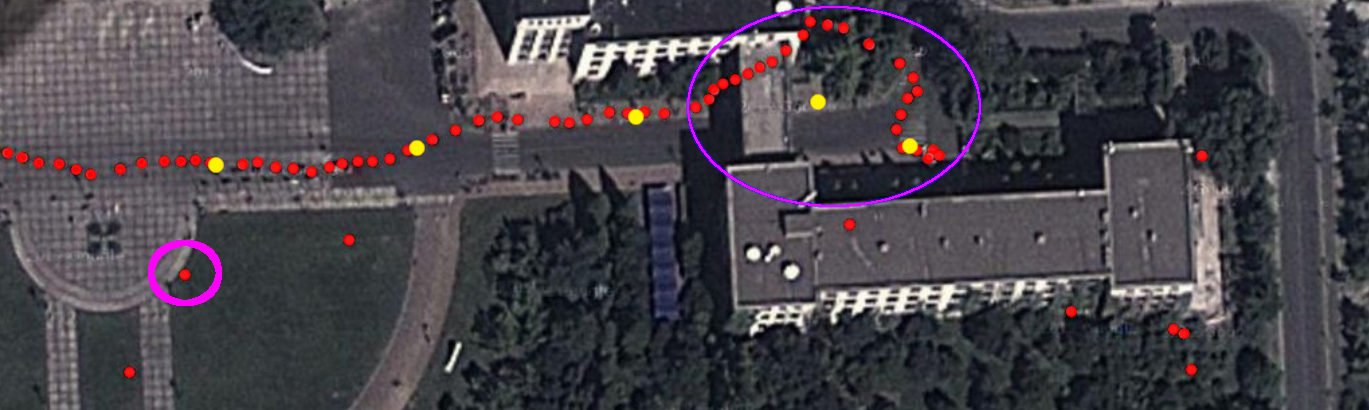
\includegraphics[width=\textwidth]{markierte_GPS_Motivation_Example.png}
    \caption{GPS-Tracking mit markierten Werte auf dem Campus der Tsinghua Universit�t}
\end{figure}
\end{frame}



\subsection{Zielsetzung}

\begin{frame}{\insertsubsection}
  \begin{block}<+->{Ziel der Arbeit}
    \begin{itemize}
      \item Einfliessen der markierten Werte in die Anomalienerkennung
            \begin{itemize}
                \item lange Folgen von Ausrei�er sollen identifiziert werden
            \end{itemize}
      \item Anomalienerkennung mit den Minimum-Change-Prinzip vereinbaren   
            \begin{itemize}
                \item keine drastische Ver�nderungen der Messwerte
            \end{itemize}
      \item Einfliessen der markierten Werte in die anderen State-of-Art Verfahren
      \item Neues Verfahren mit den anderen Verfahren empirisch vergleichen
    \end{itemize}
  \end{block}
\end{frame}


